\chapter{Realizzazione fisica delle porte logiche}
\label{ch:porte-logiche}
\textit{(6 marzo 2026)}

\section{Esercizio: bit di parità a 4 bit}

\textit{Progettare un circuito che calcoli il bit di parità di un numero a 4 bit. Il bit di parità è 0 se il numero di 1 nel numero è pari, 1 se è dispari.}

\medskip
\noindent\textbf{Come si risolve (ragionamento passo per passo):}

\begin{enumerate}[leftmargin=1.5em]
    \item \textbf{Capire cosa serve (e perché può sembrare invertita).}
    L'obiettivo della \textbf{parità pari} è che il numero \emph{totale} di $1$ trasmessi (dato $+$ bit $P$) sia sempre \textbf{pari}. Di conseguenza:
    \begin{itemize}
        \item se nel dato ci sono già un numero \textbf{pari} di $1$ $\Rightarrow$ non serve aggiungere nulla $\Rightarrow P = 0$;
        \item se nel dato ci sono un numero \textbf{dispari} di $1$ $\Rightarrow$ bisogna aggiungere un $1$ per bilanciare $\Rightarrow P = 1$.
    \end{itemize}
    \textit{Attenzione}: $P = 1$ \textbf{non} significa ``va tutto bene'', significa ``ho dovuto correggere la parità''. Detto in modo diretto: $P$ vale $1$ quando il conteggio degli $1$ nel dato è \textbf{dispari} (e dunque serviva un $1$ extra per renderlo pari).

    \item \textbf{Riconoscere la porta giusta.} Ricordiamo la tabella dello \textbf{XOR} a 2 ingressi:
    \begin{center}
    \begin{tabular}{cc|c|l}
    \toprule
    $A$ & $B$ & $A \oplus B$ & Significato \\
    \midrule
    0 & 0 & 0 & zero uni $\Rightarrow$ pari \\
    0 & 1 & 1 & un uno $\Rightarrow$ dispari \\
    1 & 0 & 1 & un uno $\Rightarrow$ dispari \\
    1 & 1 & 0 & due uni $\Rightarrow$ pari \\
    \bottomrule
    \end{tabular}
    \end{center}
    Lo XOR vale $1$ esattamente quando il numero di $1$ in ingresso è \textbf{dispari}: è dunque il componente perfetto per calcolare la parità!

    \item \textbf{Estendere a 4 bit con la proprietà associativa.} Lo XOR è \textbf{associativo}, quindi possiamo calcolare la parità su più bit applicandolo in cascata, come somma modulo 2:
    \[
        P = I_3 \oplus I_2 \oplus I_1 \oplus I_0
    \]
    Il risultato vale $1$ se e solo se il numero totale di $1$ tra i 4 bit è dispari (esattamente ciò che vogliamo).

    \item \textbf{Costruire il circuito.} Uno XOR accetta solo 2 ingressi, quindi si procede \textbf{a coppie}:
    \begin{itemize}
        \item Primo livello: $X_A = I_1 \oplus I_0$ e $X_B = I_3 \oplus I_2$ (due porte XOR in parallelo).
        \item Secondo livello: $P = X_A \oplus X_B$ (una porta XOR che combina i risultati parziali).
    \end{itemize}
    Servono quindi \textbf{3 porte XOR} in totale.

    \item \textbf{Verifica numerica.} Prendiamo $N = 1011$:
    \begin{itemize}
        \item Conta degli uni: tre $1$ $\Rightarrow$ dispari $\Rightarrow$ ci aspettiamo $P = 1$.
        \item Calcolo: $X_A = 1 \oplus 1 = 0$, $\quad X_B = 1 \oplus 0 = 1$, $\quad P = 0 \oplus 1 = 1$ \checkmark
    \end{itemize}
    Prendiamo $N = 1100$:
    \begin{itemize}
        \item Conta degli uni: due $1$ $\Rightarrow$ pari $\Rightarrow$ ci aspettiamo $P = 0$.
        \item Calcolo: $X_A = 0 \oplus 0 = 0$, $\quad X_B = 1 \oplus 1 = 0$, $\quad P = 0 \oplus 0 = 0$ \checkmark
    \end{itemize}
\end{enumerate}

\medskip
\noindent Sia $N = I_3 I_2 I_1 I_0$. Si lavora a coppie di bit, applicando lo XOR a multipli di 2:

\begin{center}
\begin{tabular}{cc|c}
\toprule
$I_3$ & $I_2$ & XOR\\
\midrule
0&0&0\\
0&1&1\\
1&0&1\\
1&1&0\\
\bottomrule
\end{tabular}
\qquad
\begin{tabular}{cc|c}
\toprule
$I_1$ & $I_0$ & XOR\\
\midrule
0&0&0\\
0&1&1\\
1&0&1\\
1&1&0\\
\bottomrule
\end{tabular}
\end{center}

Il \textbf{calcolatore di parità} si ottiene combinando in cascata 3 porte XOR:

\begin{center}
\begin{circuitikz}[scale=0.9, every node/.style={scale=0.9}]
\node[xor port] (x1) at (0,1) {};
\draw (x1.in 1) -- ++(-1,0) node[left]{$I_0$};
\draw (x1.in 2) -- ++(-1,0) node[left]{$I_1$};

\node[xor port] (x2) at (0,-1) {};
\draw (x2.in 1) -- ++(-1,0) node[left]{$I_2$};
\draw (x2.in 2) -- ++(-1,0) node[left]{$I_3$};

\node[xor port] (x3) at (2.6,0) {};
\draw (x1.out) -| (x3.in 1);
\draw (x2.out) -| (x3.in 2);
\draw (x3.out) -- ++(0.8,0) node[right]{$P$};
\end{circuitikz}
\end{center}

\section{Verifica di una trasmissione tramite parità}

Calcolando il bit di parità sia alla \textbf{partenza} ($O_1$) che all'\textbf{arrivo} ($O_2$) e confrontandoli con una porta \textbf{XNOR}, si fa passare il segnale solo se $O_1 = O_2$ (cioè $00$ oppure $11$): questo permette di controllare che il segnale non sia stato alterato durante la trasmissione.

\begin{center}
\begin{circuitikz}[scale=0.9, every node/.style={scale=0.9}]
% Block 1: Partenza (Calcolatore di parità)
\draw[thick] (0,0) rectangle (2,1.6);
\node[align=center, font=\small] at (1,0.8) {Calcolatore\\di parità};
\node[above, font=\footnotesize\bfseries] at (1,1.6) {Partenza};

% Input arrows for Block 1
\foreach \y/\label in {1.4/$I_3$, 1.1/$I_2$, 0.8/$I_1$, 0.5/$I_0$} {
  \draw[-latex] (-0.8,\y) -- (0,\y);
  \node[left, font=\scriptsize] at (-0.8,\y) {\label};
}

% XNOR Gate positioned on the right
\node[xnor port] (xn) at (8.6,0.8) {};

% Output of Block 1 (O_1) routed above Block 2 to avoid crossing
\draw[thick] (2,0.8) -- (2.4,0.8) node[above, font=\footnotesize] {$O_1$};
\draw[-latex, thick] (2.4,0.8) -- (2.4,2.2) -- (7.6,2.2) |- (xn.in 1);

% Block 2: Arrivo (Calcolatore di parità)
\draw[thick] (4.2,0) rectangle (6.2,1.6);
\node[align=center, font=\small] at (5.2,0.8) {Calcolatore\\di parità};
\node[above, font=\footnotesize\bfseries] at (5.2,1.6) {Arrivo};

% Input arrows for Block 2 (received bits, possibly with prime)
\foreach \y/\label in {1.4/$I'_3$, 1.1/$I'_2$, 0.8/$I'_1$, 0.5/$I'_0$} {
  \draw[-latex] (3.4,\y) -- (4.2,\y);
  \node[left, font=\scriptsize] at (3.4,\y) {\label};
}

% Output of Block 2 (O_2) routed to XNOR
\draw[thick] (6.2,0.8) -- (6.8,0.8) node[above, font=\footnotesize] {$O_2$};
\draw[-latex, thick] (6.8,0.8) |- (xn.in 2);

% Output of XNOR
\draw (xn.out) -- ++(0.8,0) node[right, align=left, font=\footnotesize] {Abilita se $O_1 = O_2$\\(nessun errore)};
\end{circuitikz}
\end{center}

\section{Caratteristiche fisiche delle porte logiche}

Le diverse \textbf{famiglie logiche} (RTL, DTL, HTL, TTL, ECL, MOS, CMOS) si confrontano in base a parametri come la porta di base, il fan-out, la potenza dissipata, l'immunità al rumore, il ritardo di propagazione e la frequenza massima di funzionamento. In generale:

\begin{itemize}[leftmargin=1.5em]
    \item \textbf{TTL} (Transistor-Transistor Logic): ottimo compromesso velocità/potenza, molto diffusa;
    \item \textbf{ECL} (Emitter-Coupled Logic): velocissima ma con elevato consumo;
    \item \textbf{CMOS} (Complementary Metal-Oxide-Semiconductor): bassissima potenza dissipata, oggi la più usata nei circuiti integrati.
\end{itemize}

\section{Implementazione delle porte logiche}

\subsection{NOT con un singolo transistor}

La porta NOT più semplice si realizza con un singolo transistor NPN in configurazione a emettitore comune, con una resistenza di pull-up $R_C$ verso $V_{CC}$ e una resistenza di base $R_B$ che limita la corrente di base:

\begin{center}
\begin{circuitikz}[american voltages]
\draw (0,0) node[npn](Q1){}
  (Q1.C) to[short,-*] (Q1.C -| 0,2) to[R, l=$R_C$] (Q1.C |- 0,3.5) node[above]{$V_{CC}$}
  (Q1.B) to[R, l_=$R_B$, -o] ++(-2.0,0) node[left]{$V_{in}$}
  (Q1.E) to[short] ++(0,-1) node[ground]{}
  (Q1.C) to[short,-o] ++(1.6,0) node[right]{$V_{out}$}
;
\end{circuitikz}
\end{center}

\begin{important}
\begin{itemize}[leftmargin=1.3em]
    \item $V_{in} = 5\,\text{V} \;(=1) \Rightarrow$ il transistor satura $\Rightarrow V_{out} = 0,2\,\text{V} \;(=0)$;
    \item $V_{in} = 0\,\text{V} \;(=0) \Rightarrow$ il transistor è spento $\Rightarrow V_{out} = 5\,\text{V} \;(=1)$.
\end{itemize}
\end{important}

\begin{center}
\begin{circuitikz}
\node[not port] (n1) at (0,0) {};
\draw (n1.in 1) -- ++(-0.6,0);
\draw (n1.out) -- ++(0.6,0);
\end{circuitikz}
\end{center}

\subsection{NOT in tecnologia TTL}

Nella tecnologia TTL (\emph{Transistor-Transistor Logic}), la porta logica base non utilizza singoli diodi o resistenze in ingresso, ma sfrutta i transistor bipolari (BJT) per migliorare velocità e prestazioni. La porta NOT TTL standard si divide in tre stadi principali:

\begin{enumerate}[leftmargin=1.5em]
    \item \textbf{Stadio di ingresso}: utilizza un transistor NPN ($Q_1$) in cui l'emettitore funge da ingresso. Se l'ingresso è basso ($0\,\mathrm{V}$), $Q_1$ va in conduzione portando a massa la base dello stadio successivo. Se l'ingresso è alto ($5\,\mathrm{V}$), la giunzione base-emettitore è polarizzata inversamente e la corrente fluisce verso la base del driver.
    \item \textbf{Sfasatore (driver)}: il transistor centrale ($Q_2$) riceve il segnale da $Q_1$ e pilota in controfase i due transistor finali. Produce due segnali logici opposti: uno al collettore e uno all'emettitore.
    \item \textbf{Stadio di uscita a totem-pole}: costituito da due transistor ($Q_3$ e $Q_4$) impilati uno sull'altro e un diodo. Garantisce un'uscita ``forte'' a bassa impedenza in entrambi gli stati logici: $Q_3$ spinge attivamente l'uscita a livello alto (pull-up attivo), mentre $Q_4$ la tira a massa (pull-down). Il diodo aggiunge una caduta di tensione che garantisce che $Q_3$ resti spento quando $Q_4$ è in saturazione. Durante le commutazioni i due transistor possono condurre brevemente insieme: il resistore da $130\,\Omega$ limita il picco di corrente che ne deriva.
\end{enumerate}

\begin{center}
\begin{circuitikz}[american voltages, scale=0.85, every node/.style={scale=0.85}]
\draw (0,4.5) -- (7,4.5);
\node[above] at (3.5,4.5) {$V_{CC} \ (+5\,\mathrm{V})$};

% R1
\draw (1,4.5) to[R=$4\,\mathrm{k}\Omega$] (1,2.5) coordinate (bQ1);
% R2
\draw (3.5,4.5) to[R=$1.6\,\mathrm{k}\Omega$] (3.5,2.5) coordinate (cQ2);
% R4
\draw (5.5,4.5) to[R=$130\,\Omega$] (5.5,3.2) coordinate (cQ3);

% Q1
\node[npn] (Q1) at (1.5,1.7) {};
\node at ($(Q1.C)+(0.4,0)$) {$Q_1$};
\draw (bQ1) -| (Q1.B);
\draw (Q1.E) -- ++(-1.5,0) to[short,-o] ++(0,0) node[left]{$V_{in}$};

% Q2
\node[npn] (Q2) at (3.5,1.7) {};
\node at ($(Q2.C)+(0.4,0.1)$) {$Q_2$};
\draw (Q1.C) |- (Q2.B);
\draw (cQ2) -- (Q2.C);

% Q2 emitter resistor
\draw (Q2.E) to[R=$1\,\mathrm{k}\Omega$] ++(0,-1.5) node[ground]{};

% Q3
\node[npn] (Q3) at (5.5,2.4) {};
\node at ($(Q3.C)+(0.4,0)$) {$Q_3$};
\draw (cQ3) -- (Q3.C);
\draw (Q2.C) |- (Q3.B);

% Diode
\draw (Q3.E) to[D] ++(0,-1) coordinate (dout);

% Q4
\node[npn] (Q4) at (5.5,0.6) {};
\node at ($(Q4.C)+(0.4,0)$) {$Q_4$};
\draw (dout) -- (Q4.C);
\draw (Q2.E) |- (Q4.B);
\draw (Q4.E) -- ++(0,-0.3) node[ground]{};

% Vout
\draw (dout) to[short,-o] ++(1.5,0) node[right]{$V_{out}$};

% Labels for stages
\node[align=center, font=\footnotesize, text=blue!80!black] at (1,-0.5) {Stadio di\\ingresso};
\node[align=center, font=\footnotesize, text=blue!80!black] at (3.5,-0.5) {Sfasatore\\(Driver)};
\node[align=center, font=\footnotesize, text=blue!80!black] at (6.2,-0.5) {Uscita a\\Totem-Pole};

% Dashed lines separating stages
\draw[dashed, gray] (2.5, 4.5) -- (2.5, -1);
\draw[dashed, gray] (4.5, 4.5) -- (4.5, -1);

\end{circuitikz}
\end{center}

\section{Immunità al rumore}

L'immunità al rumore di un sistema digitale non è totale, ma è comunque molto più elevata di quella dei sistemi analogici, perché due porte in cascata ``ripuliscono'' il segnale ad ogni passaggio rigenerando i livelli di tensione:

\begin{center}
\begin{circuitikz}
\node[buffer port] (b1) at (0,0) {};
\node[buffer port] (b2) at (2,0) {};
\draw (b1.in 1) -- ++(-0.6,0) node[left]{in};
\draw (b1.out) -- (b2.in 1);
\node[above] at ($(b1.out)!0.5!(b2.in 1)$) {\footnotesize out$'$/in$'$};
\draw (b2.out) -- ++(0.6,0) node[right]{out$''$};
\end{circuitikz}
\end{center}

Per garantire il corretto riconoscimento dei livelli logici, i costruttori definiscono le soglie di tensione per l'ingresso e l'uscita:

\begin{important}
\begin{minipage}{0.48\linewidth}
\textbf{Livello alto (High)}
\begin{itemize}[leftmargin=1.3em]
    \item $V_{OH,min}$: $V_{out}$ minima garantita per l'uscita alta;
    \item $V_{OH,max}$: $V_{out}$ massima possibile per l'uscita alta;
    \item $V_{IH,min}$: $V_{in}$ minima richiesta in ingresso per essere letta come alta;
    \item $V_{IH,max}$: $V_{in}$ massima ammessa per un ingresso alto.
\end{itemize}
\end{minipage}
\hfill
\begin{minipage}{0.48\linewidth}
\textbf{Livello basso (Low)}
\begin{itemize}[leftmargin=1.3em]
    \item $V_{OL,min}$: $V_{out}$ minima possibile per l'uscita bassa;
    \item $V_{OL,max}$: $V_{out}$ massima garantita per l'uscita bassa;
    \item $V_{IL,min}$: $V_{in}$ minima ammessa per un ingresso basso;
    \item $V_{IL,max}$: $V_{in}$ massima tollerata in ingresso per essere letta come bassa.
\end{itemize}
\end{minipage}
\end{important}

La differenza tra le tensioni garantite in uscita e quelle minime/massime tollerate in ingresso definisce i \textbf{margini di rumore} (\emph{noise margin}):
\[
NM_H = V_{OH,min} - V_{IH,min} \qquad\qquad
NM_L = V_{IL,max} - V_{OL,max}
\]
I margini di rumore ($NM_H$ e $NM_L$) rappresentano l'ampiezza massima di un disturbo (rumore elettrico, fluttuazioni) che può sommarsi al segnale durante il tragitto lungo il filo senza far sì che la porta successiva lo interpreti in modo errato o lo collochi nella \emph{zona proibita}. In altre parole, è il ``cuscinetto di sicurezza'' contro il rumore.

\begin{center}
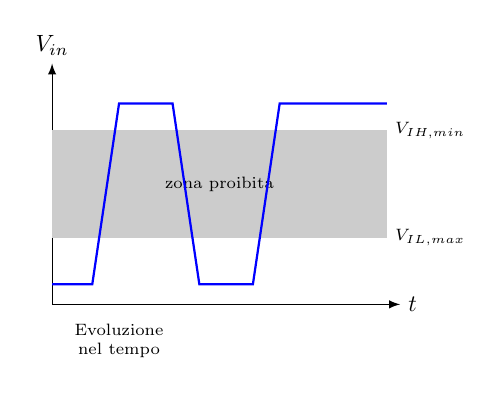
\begin{tikzpicture}[scale=0.85, every node/.style={scale=0.85}]
% --- grafico 1: zona proibita nel tempo ---
\draw[-latex] (0,0) -- (5.2,0) node[right]{$t$};
\draw[-latex] (0,0) -- (0,3.6) node[above]{$V_{in}$};
\draw[dashed] (0,2.6) -- (5,2.6) node[right,font=\scriptsize]{$V_{IH,min}$};
\draw[dashed] (0,1.0) -- (5,1.0) node[right,font=\scriptsize]{$V_{IL,max}$};
\filldraw[gray!40] (0,1.0) rectangle (5,2.6);
\node[font=\scriptsize] at (2.5,1.8) {zona proibita};
\draw[thick,blue] (0,0.3) -- (0.6,0.3) -- (1.0,3.0) -- (1.8,3.0) -- (2.2,0.3) -- (3.0,0.3) -- (3.4,3.0) -- (5,3.0);
\node[font=\scriptsize, align=center] at (1.0,-0.55) {Evoluzione\\nel tempo};
\end{tikzpicture}
\qquad
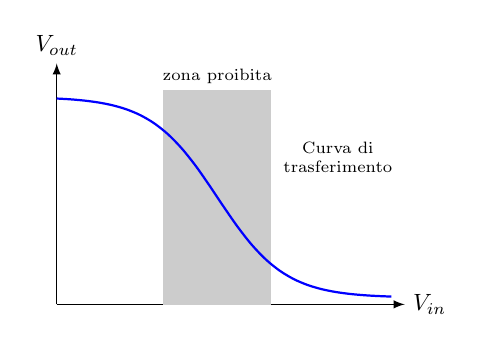
\begin{tikzpicture}[scale=0.85, every node/.style={scale=0.85}]
% --- grafico 2: funzione di trasferimento ---
\draw[-latex] (0,0) -- (5.2,0) node[right]{$V_{in}$};
\draw[-latex] (0,0) -- (0,3.6) node[above]{$V_{out}$};
\filldraw[gray!40] (1.6,0) rectangle (3.2,3.2);
\node[font=\scriptsize] at (2.4,3.4) {zona proibita};
\draw[thick,blue,domain=0:5,smooth] plot (\x,{3.0/(1+exp(2*(\x-2.4)))+0.1});
\node[font=\scriptsize, align=center] at (4.2,2.2) {Curva di\\trasferimento};
\end{tikzpicture}
\end{center}

\noindent\textbf{Cosa rappresentano i due grafici:}
\begin{itemize}[leftmargin=1.5em]
    \item \textbf{Grafico di sinistra (Evoluzione nel tempo):} Mostra come varia nel tempo la tensione in ingresso ($V_{in}$) ad una porta. La fascia grigia è la \textbf{zona proibita}: se la tensione cade in quest'area, il componente \emph{non può} stabilire se il livello logico sia uno $0$ o un $1$. I fronti di salita e discesa del segnale devono attraversare questa zona il più rapidamente possibile.
    \item \textbf{Grafico di destra (Curva di trasferimento):} È il grafico $V_{out}$ in funzione di $V_{in}$ (es. per un inverter NOT). Un inverter ideale commuterebbe a gradino esatto, ma nella realtà c'è una pendenza. Mostra chiaramente che finché $V_{in}$ resta \emph{fuori} dalla zona proibita grigia (a sinistra o a destra), $V_{out}$ assume un valore netto e stabile ai margini del grafico logico.
\end{itemize}

\section{Nomenclatura delle famiglie logiche e fan-out}

\subsection{Nomenclatura dei componenti}
Le sigle dei circuiti integrati logici (IC) commerciali seguono uno schema di identificazione ben preciso. Ad esempio, una porta \textbf{SN74LS00N} viene così codificata:
\[
\underbrace{SN}_{\text{ditta produttrice}}\;\underbrace{74}_{\text{famiglia logica}}\;\underbrace{LS}_{\text{sotto-famiglia}}\;\underbrace{00}_{\text{funzione}}\;\underbrace{N}_{\text{package}}
\]
In dettaglio:
\begin{itemize}[leftmargin=1.5em]
    \item \textbf{Ditta produttrice}: ad esempio \emph{SN} per Texas Instruments, \emph{MC} per Motorola.
    \item \textbf{Famiglia logica / range temperature}: la famiglia \textbf{74} è per uso commerciale ($0^\circ\text{C} \div 70^\circ\text{C}$), mentre la \textbf{54} è per uso militare/aerospaziale con tolleranze molto più ampie ($-55^\circ\text{C} \div 125^\circ\text{C}$).
    \item \textbf{Sotto-famiglia (tecnologia)}: specifica le caratteristiche di velocità e consumi. Ad esempio \emph{LS} (Low-power Schottky), \emph{HC} (High-speed CMOS), \emph{ALS} (Advanced Low-power Schottky).
    \item \textbf{Funzione}: il codice \emph{00} indica ad esempio ``Quad 2-input NAND gate'' (4 porte NAND a due ingressi), \emph{04} indica un \emph{hex inverter} (6 porte NOT nello stesso integrato), ecc.
    \item \textbf{Package}: indica il tipo di contenitore fisico del chip. Ad esempio la lettera \emph{N} indica il classico package plastico DIP (Dual In-line Package) per fori passanti, \emph{D} indica un package SOIC per montaggio superficiale.
\end{itemize}

\subsection{Fan-Out (capacità di pilotaggio)}

\begin{definizione}{Fan-Out}
numero massimo di ingressi di porte logiche uguali che l'uscita di una determinata porta è in grado di pilotare, garantendo i corretti livelli di tensione.
\end{definizione}

Perché c'è un limite? Ogni porta in ingresso assorbe (o eroga) una piccolissima quantità di corrente. Se colleghiamo troppe porte all'uscita di un'unica porta ``driver'', la somma di queste piccole correnti diventa elevata. Se il driver non è progettato per erogare tutta questa corrente, la sua tensione di uscita inizia ad abbassarsi (o alzarsi) finendo nella zona proibita e causando errori nel circuito.

Il calcolo del Fan-Out si effettua separatamente per i due stati logici Alto e Basso, prendendo poi il caso peggiore (il minimo tra i due calcoli):
\[
FO_H = \dfrac{I_{out,H}}{I_{in,H}} \qquad\qquad
FO_L = \dfrac{I_{out,L}}{I_{in,L}}
\]

Nello schema seguente è illustrato il concetto: la corrente totale $I_{out}$ che fuoriesce dalla porta ``Driver'' si divide in tante piccole $I_{in}$ quanti sono i carichi. Tutta la rete di carichi può essere modellata teoricamente come un'unica resistenza equivalente verso massa o verso l'alimentazione:

\begin{center}
\begin{circuitikz}[scale=0.9, every node/.style={scale=0.9}]
% Driving gate
\node[not port] (drv) at (0,0) {};
\node[above] at (drv) {Driver};
\draw (drv.in 1) -- ++(-0.6,0) node[left]{$V_{in}$};

% Split node
\coordinate (split) at (1.5,0);
\draw (drv.out) -- (split);
\draw[-latex] (drv.out) -- ++(0.7,0) node[above]{$I_{out}$};

% Load gates
\node[not port] (L1) at (3.5,1.2) {};
\node[not port] (L2) at (3.5,0) {};
\node[not port] (Ln) at (3.5,-1.5) {};

\node[right] at (L1.out) {Carico 1};
\node[right] at (L2.out) {Carico 2};
\node[right] at (Ln.out) {Carico $n$};

\draw (split) |- (L1.in 1);
\draw (split) -- (L2.in 1);
\draw (split) |- (Ln.in 1);

\draw[-latex] (1.5,1.2) -- ++(0.8,0) node[above]{$I_{in,1}$};
\draw[-latex] (1.5,0) -- ++(0.8,0) node[above]{$I_{in,2}$};
\draw[-latex] (1.5,-1.5) -- ++(0.8,0) node[above]{$I_{in,n}$};

\node at (1.5,-0.7) {$\vdots$};
\node at (3.5,-0.7) {$\vdots$};

% Equivalence text
\node at (6.2, 0) {\Large $\equiv$};

% Equivalent circuit
\node[not port] (eqdrv) at (8.5,0) {};
\draw (eqdrv.in 1) -- ++(-0.6,0);
\draw (eqdrv.out) -- ++(0.5,0) coordinate (eqsplit);
\draw (eqsplit) to[R, l=$R_{eq}$] ++(0,-1.5) node[ground]{};
\node[above] at (eqdrv) {Driver};

\end{circuitikz}
\end{center}

% ======================================================================
\section*{Riepilogo del Capitolo}

\begin{important}
Le porte logiche si realizzano fisicamente con transistor (es. TTL a tre stadi con uscita totem-pole); la qualità elettrica dell'interfacciamento fra porte reali si misura con i \textbf{margini di rumore} e il \textbf{fan-out}, non con il solo comportamento ideale 0/1.
\end{important}

\begin{note}
\textbf{Regole fondamentali:}
\begin{itemize}
    \item \textbf{Margini di rumore:} $NM_H = V_{OH,min}-V_{IH,min}$, $\; NM_L = V_{IL,max}-V_{OL,max}$.
    \item \textbf{Fan-Out:} $FO_H = I_{out,H}/I_{in,H}$, $\; FO_L = I_{out,L}/I_{in,L}$ (si considera il minimo tra i due).
    \item \textbf{Calcolatore di parità a 4 bit:} $P = I_3 \oplus I_2 \oplus I_1 \oplus I_0$ (cascata di porte XOR, per associatività).
    \item \textbf{Famiglie logiche:} TTL (compromesso velocità/potenza), ECL (veloce, alto consumo), CMOS (bassissima potenza, oggi predominante).
\end{itemize}
\end{note}

